%-*-latex-*-
\section{Bubblesort again: Computing for-loop runtime
quickly}

Let me redo the runtime analysis for the bubblesort again.
This time I'm going to show you some tricks for simplifying the 
computation of the runtime.

Remember that we're interested in the big-O of the runtime.
So ultimately, we're going to replaced constants (the coefficients
of the polynomial) by 1.
Notice that I did this simplification at the end after
computing the runtime.
Now wouldn't it be a good idea to simplify my constants
as early as possible?

Here's the algorithm with times for each statement:
With time for each statement:
\begin{Verbatim}[frame=single, fontsize=\footnotesize]
          i = n - 2               t1
LOOP1:    if i == -1:             t2
              goto ENDLOOP1       t3

              j = 0               t4
LOOP2:        if j > i:           t5
                  goto ENDLOOP2   t6
              if a[i] < a[j + 1]: t7
                  t = a[i]        t8
                  a[i] = a[j]     t9
                  a[j] = t        t10
              j = j + 1           t11
              goto LOOP2          t12

ENDLOOP2: i = i - 1               t13
          goto LOOP1              t14

ENDLOOP1:
\end{Verbatim}
I'm going to analyze the worst case again.

The runtime computation in the previous section 
was rather long.
So I'm going to try to simplify it in several ways.

\begin{itemize}

\li The first question to ask is this: Can we stick to the for-loop
    without using goto statements? Converting to the format with goto
statement increases the number of statements to time.
Can we avoid that?

\li The second question is this:
The big-O allows us to simplify the runtime
function by throwing away constants (or rather replace them by 1).
Why not perform this simplification step earlier?
Another simplification done during big-O computation is that
we retain the part (i.e. the term) that grows the fastest.
Can we do that earlier too? In other words can we using
big-O fudging as early as possible instead of at the last stage?

\li The third question will only appear after I've addressed the above two.
Once the simplification techniques above are addressed,
you will see that runtime computations will become a lot simpler if there
standard formulas. A minor point is that I will show you that 
the big-O of certain summations are not not changed if the lower and upper 
limits of the sum is changed by a constant amount.

\end{itemize}

Let's start with a simple for-loop ...
let's look at the inner loop of the bubblesort which depends on $i$:
\begin{Verbatim}[frame=single, fontsize=\footnotesize]
...
              j = 0               t4   1
LOOP2:        if j > i:           t5   i + 1
                  goto ENDLOOP2   t6   1
              if a[i] < a[j + 1]: t7   i
                  t = a[i]        t8   i
                  a[i] = a[j]     t9   i
                  a[j] = t        t10  i
              j = j + 1           t11  i
              goto LOOP2          t12  i

ENDLOOP2: 
...
\end{Verbatim}
The body of the inner loop is this:
\begin{Verbatim}[frame=single, fontsize=\footnotesize]
              if a[i] < a[j + 1]: t7   i
                  t = a[i]        t8   i
                  a[i] = a[j]     t9   i
                  a[j] = t        t10  i
\end{Verbatim}
Let's call this runtime function $U(i)$.
The runtime is
\begin{align*}
U(i) 
&= t_4 + (i + 1)t_5 + t_6 + i(t_7 + t_8 + t_9 + t_{10} + t_{11}) \\
&= (t_5 + t_7 + t_8 + t_9 + t_{10} + t_{11})i + (t_4 + t_5 + t_6) \\
&= Ai + B
\end{align*}
for constants $A$ and $B$. 
Phew! What a pain to compute!

Now I know that the body of the inner loop is constant time.
When I'm computing time, I don't really care about the actual
statements.
So I will give the body a time of 
\verb!t13! and view the inner loop like this:
\begin{Verbatim}[frame=single, fontsize=\footnotesize]
...
              j = 0               t4   1
LOOP2:        if j > i:           t5   i + 1
                  goto ENDLOOP2   t6   1
              [BODY BLOCK]        t13  i
              j = j + 1           t11  i
              goto LOOP2          t12  i

ENDLOOP2: 
...
\end{Verbatim}
Of course $U(i)$ becomes:
\begin{align*}
U(i) 
&= t_4 + (i + 1)t_5 + t_6 + i(t_{13} + t_{11}) \\
&= (t_5 + t_{13} + t_{11})i + (t_4 + t_5 + t_6) \\
&= Ai + B
\end{align*}
Well ... the computation sure looks slightly simpler.

So the basic principle here is this:
collapse chunks of statements into a block and assign
a single time to that block will simplify the computation
a little.

Analogous to this is that whenever you have constant expression
you might want to rename it with a symbol.
For instance in the above computation, you might write:
\begin{align*}
U(i) 
&= t_4 + (i + 1)t_5 + t_6 + i(t_{13} + t_{11}) \\
&= A + (i + 1)t_5 + iB \hspace{1in} \text{ for some constants $A$, $B$}\\
&= ...
\end{align*}
In this case of course $A = t_4 + t_6$ and $B = t_{13} + t_{11}$.



Let's redo the above in two piece.
The computation of $U(i)$ is made up the time to execute the
body of the loop and the time taken for the for-loop
to control the execution of the body.


So now I want look at the \lq\lq loop control'', i.e., the code that
is in charge of repeating the body for the correct number of times:
\begin{Verbatim}[frame=single, fontsize=\footnotesize]
...
              j = 0               t4   1
LOOP2:        if j > i:           t5   i + 1
                  goto ENDLOOP2   t6   1
              ...
              j = j + 1           t11  i
              goto LOOP2          t12  i

ENDLOOP2: 
...
\end{Verbatim}

Next, I'm going to bunch up \verb!t11! and \verb!t12!:
\begin{Verbatim}[frame=single, fontsize=\footnotesize]
...
              j = 0                    t4   1
LOOP2:        if j > i:                t5   i + 1
                  goto ENDLOOP2        t6   1
              ...
              j = j + 1; goto LOOP2    t15  i

ENDLOOP2: 
...
\end{Verbatim}
You see immediately that the time taken for the \lq\lq loop control''
is
\begin{align*}
\text{LOOP CONTROL TIME} 
&= 
t_4 + 
(i + 1) t_5 + 
t_6 + 
i t_{15}
\\
&= A(i+1) + B
\end{align*}
where $A$ \textit{ includes} 
the time taken to compute the boolean expression.
Note that if the body runs $i$ times, then the boolean
expresssion is computed $i + 1$ times.
If $A$ is a constant
\begin{align*}
\text{LOOP CONTROL TIME} 
&= Ai + (A + B) \\
&= (A + 1)i + B \\
&= Ci + B
\end{align*}
for constants $A$, $B$, and $C$.
Let me summarize this fact and call it TRICK1:


\textbf{TRICK1.}
The total runtime of
\begin{Verbatim}[frame=single, fontfamily=tt, fontsize=\footnotesize]
for i = 1, 2, ..., n:             
    [body(i)]                     Time to run body(i)
\end{Verbatim}
is of the form 
\[
\sum_{i=1}^n (\text{Time to execute body($i$))} + An + B 
\]
where $A$ and $B$ are constants.
In general the total runtime of
\begin{Verbatim}[frame=single, fontfamily=tt, fontsize=\footnotesize]
for i = m, 2, ..., n:             
    [body(i)]                     Time to run body(i)
\end{Verbatim}
is of the form 
\[
\sum_{i=m}^n (\text{Time to execute body($i$))} + A(n-m+1) + B 
\]
(Of course $n-m+1$ is the number of times the body of the
loop is executed.)


Back to our bubblesort \textit{ without goto statements} and
here's the second solution ...

\newpage

\begin{eg}
Compute the worst runtime of the bubblesort:
\begin{Verbatim}[frame=single, fontsize=\footnotesize]
for i = n - 2, ..., 0:
    for j = 0, ..., i:
        if a[i] > a[i + 1]:
            t = a[i]
            a[i] = a[i + 1]
            a[i + 1] = t
\end{Verbatim}
\end{eg}

\textit{ Solution.}
The inner most body 
\begin{Verbatim}[frame=single, fontsize=\footnotesize]
        if a[i] > a[i + 1]:
            t = a[i]
            a[i] = a[i + 1]
            a[i + 1] = t
\end{Verbatim}
has constant runtime, say $A$.
Let $U(i)$ be the runtime of the inner for-loop.
Using TRICK1, since the inner loop runs $i + 1$ times:
\[
U(i) = \sum_{j=0}^i A + B(i+1) + C = A(i+1) + B(i+1) + C = Di + E
\]
for constants $A, B, C, D, E$.
Using TRICK1 again, since the outer loop runs $n - 1$ times
the whole algorithm has a runtime of
\[
T(n) = \sum_{i=0}^{n-2} U(i) + F(n-1) + G
\]
Therefore
\begin{align*}
T(n) 
&= \sum_{i=0}^{n-2} (Di + E) + F(n-1) + G \\
&= D \sum_{i=0}^{n-2} i + E \sum_{i=0}^{n-2} 1 + F(n-1) + G \\
&= D \frac{(n-2)(n-1)}{2}  + E(n-1) + F(n-1) + G \\
&= \left(\frac{D}{2}\right) n^2 
   + \left( 
       -\frac{3D}{2} + E + F \right)n + \left(D - E - F + G
     \right) \\
&=O (n^2)
\end{align*}
\qed

\newpage

Note that the above big-O computation does not require goto statements
and massive number of statement counting.
The solution is definitely simpler and less error prone.

Not only that, this method also allows you to see very quickly
that the best case is also $O(n^2)$.
I'll leave that as an exercise for you.

From the computation of the above
example, you should see this one coming ...

\textbf{ADVICE:} For nested loops, try to  
compute the runtime by working from the innermost loop to the outmost.


[Despite what some intro books say, this is \textit{ not} always a good idea.
But this is something you should try if you do see nested loops.]


\begin{ex}
Compute the best runtime of the bubblesort.
\qed
\end{ex}

\begin{ex}
Show that the big-O of the runtime of the following is $O(n)$.
\begin{Verbatim}[frame=single, fontsize=\footnotesize]
for i = 0, ..., n - 1:
    x[i] = i
for i = 0, ..., n - 2:
    x[i] = x[i] + x[i + 1]
\end{Verbatim}
\qed
\end{ex}

\begin{ex}
Show that the big-O of the runtime the following is $O(n)$.
\begin{Verbatim}[frame=single, fontsize=\footnotesize]
for i = 0, ..., n - 1:
    x[i] = i
x[0] = 42
for i = n - 1, ..., 2:
    x[i] = x[i - 1] + x[i - 2]
\end{Verbatim}
\qed
\end{ex}


\begin{ex}
Show that the big-O of the runtime of the following is $O(n)$.
\begin{Verbatim}[frame=single, fontsize=\footnotesize]
for i = 0, ..., n - 1:
    x[i] = i
for i = 0, ..., n - 1:
    x[i] = x[i] * x[i]
\end{Verbatim}
\qed
\end{ex}


\begin{ex}
Compute the big-O of the runtime of the following:
\begin{Verbatim}[frame=single, fontsize=\footnotesize]
for i = 0,...,n - 1:
    x[i] = i
for i = 0, ..., n - 1:
    for j = 0, ..., i:
        x[i] = x[i] * x[i]
\end{Verbatim}
\qed
\end{ex}


\begin{ex}
Compute the big-O of the runtime of the folllowing:
\begin{Verbatim}[frame=single, fontsize=\footnotesize]
for i = 0, ..., n - 1:
    for j = 0, ..., n - 1:
        x[i] = x[i] * x[i]
\end{Verbatim}
\qed
\end{ex}


\begin{ex}
Compute the big-O of the runtime of the folllowing:
\begin{Verbatim}[frame=single, fontsize=\footnotesize]
for i = 0, ..., n - 1:
    for j = 0, ..., (n - 1) / 2:
        x[i] = x[i] * x[i]
\end{Verbatim}
Note that in the above expression \verb!(n - 1)/2!, 
I mean the floor of \verb!(n - 1)/2!.
In your computation, you can ignore floors and ceilings, 
i.e., your computations, the ceiling or floor of $n / d$ can be
replaced by $n / d$.
\qed
\end{ex}

\begin{ex}
Compute the big-O of the runtime of the following:
\begin{Verbatim}[frame=single, fontsize=\footnotesize]
for i = 0, ..., n - 1:
    for j = i, ..., (n - 1) / 2:
        x[i] = x[i] * x[i]
\end{Verbatim}
\qed
\end{ex}

\begin{ex}
What is the big-O of runtime of the following:
\begin{Verbatim}[frame=single, fontsize=\footnotesize]
for i = 0, 1, 2, ..., n - 1:
    if n is even:
        x[i] = 0
    else:
        x[i] = 1
\end{Verbatim}
\end{ex}



\begin{ex}
What is the best and worst case big-O of the following:
\begin{Verbatim}[frame=single, fontsize=\footnotesize]
for i = 0, 1, 2, ..., n - 1:
    if x[i] is even:
        for j = i + 1, ..., n - 1:
            x[i] = x[i] + x[j]
    else:
        x[i] = 0
\end{Verbatim}
\end{ex}


\begin{ex}
What is the big-O of the following:
\begin{Verbatim}[frame=single, fontsize=\footnotesize]
for i = 0, 1, 2, ..., n - 1:
    for j = 0, 1, 2, ..., i:
        x[i] = i * x[j] 
\end{Verbatim}
\end{ex}


\begin{ex}
What is the big-O of the following:
\begin{Verbatim}[frame=single, fontsize=\footnotesize]
for i = 0, 1, 2, ..., n - 1:
    for j = i + 1, ..., n * n;
        x[i] = x[i] + j * j;
\end{Verbatim}
\end{ex}


\begin{ex}
What is the big-O of the runtime of the following:
\begin{Verbatim}[frame=single, fontsize=\footnotesize]
for i = 0, 1, 2, ..., n - 1:
    x[i] = x[i] * x[i]
    for j = 0, 1, 2, ..., n - 1:
        x[j] = x[i] + i 
        for k = 0, 1, 2, ..., n - 1:
            x[k] = x[i] + x[j] + x[k]
    x[i] = x[i] - 1
\end{Verbatim}
\end{ex}


\begin{ex}
What is the big-O of the best and worst case of the following:
\begin{Verbatim}[frame=single, fontsize=\footnotesize]
for i = 0, 1, 2, ..., n - 1:
    if x[i] is even:
        for j = 0, 1, 2, ..., i:
            for k = 0, 1, 2, ..., j:
                x[k] = x[j] + x[i]
\end{Verbatim}
\end{ex}


\begin{ex}
What is the big-O of the best and worst case of the following:
\begin{Verbatim}[frame=single, fontsize=\footnotesize]
for i = 0, 1, 2, ..., n - 2:
    x[i] = x[i + 1]
    for j = 0, 1, 2, ..., i:
        if j is even:
            x[j] = x[i] + 1
        else:
            x[j] = x[i] - 1
        for k = n - 1, n - 2, ..., j:
            x[k] = x[j] + x[i]
\end{Verbatim}
\end{ex}



Of course in general the runtime of the body of the for loop
might not be a constant.
For instance: 
\begin{Verbatim}[frame=single, fontsize=\footnotesize]
for i = 0, 1, 2, 3, ..., n - 1:
    f(i, n)
\end{Verbatim}
where $f$ is a function.

Note that the case where the runtime 
of the innermost body of a loop is constant
(or at least easy to compute) and where the number of times the body
is executed is simple (example: $i$ runs from $0$ to $n-1$),
the runtime of the whole algorithm is usually pretty easy to compute.

However if you do not know how many times the body of a loop is executed,
then it's not so simple.
Here's an example:
\begin{Verbatim}[frame=single, fontsize=\footnotesize]
while n > 1:
    if n is even:
        n = n / 2
    else:
        n = 3 * n + 1
\end{Verbatim}
You can try to compute it several cases by hand.
Here's the plot of the number of iterations of the body of the while loop
for $n = 1, ..., 19$:
\begin{center}
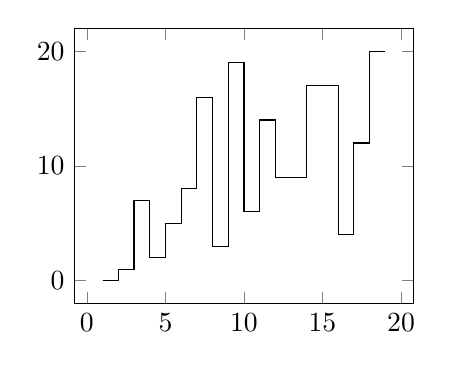
\begin{tikzpicture}
\begin{axis}[height=2in]
\addplot[const plot, no markers] coordinates {
(1,0)
(2,1)
(3,7)
(4,2)
(5,5)
(6,8)
(7,16)
(8,3)
(9,19)
(10,6)
(11,14)
(12,9)
(13,9)
(14,17)
(15,17)
(16,4)
(17,12)
(18,20)
(19,20)
};
\end{axis}
\end{tikzpicture}
\end{center}
Not so clear, right?
Here's the plot for $n = 1, ..., 99$:
\begin{center}
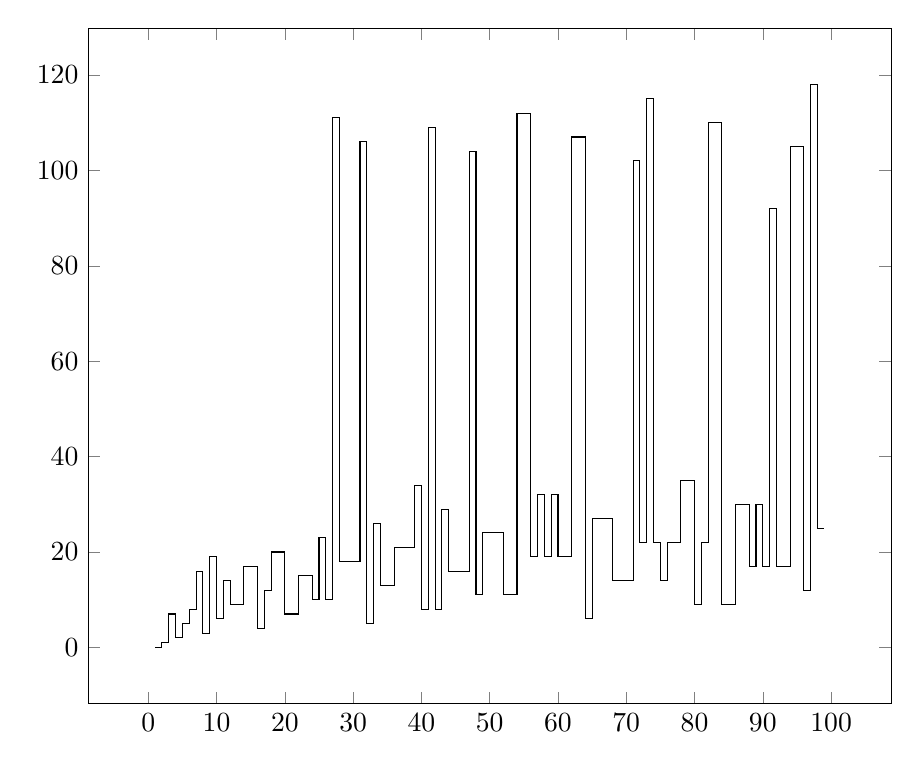
\begin{tikzpicture}
\begin{axis}[height=4in]
\addplot[const plot, no markers] coordinates {(1,0)(2,1)(3,7)(4,2)(5,5)(6,8)(7,16)(8,3)(9,19)(10,6)(11,14)(12,9)(13,9)(14,17)(15,17)(16,4)(17,12)(18,20)(19,20)(20,7)(21,7)(22,15)(23,15)(24,10)(25,23)(26,10)(27,111)(28,18)(29,18)(30,18)(31,106)(32,5)(33,26)(34,13)(35,13)(36,21)(37,21)(38,21)(39,34)(40,8)(41,109)(42,8)(43,29)(44,16)(45,16)(46,16)(47,104)(48,11)(49,24)(50,24)(51,24)(52,11)(53,11)(54,112)(55,112)(56,19)(57,32)(58,19)(59,32)(60,19)(61,19)(62,107)(63,107)(64,6)(65,27)(66,27)(67,27)(68,14)(69,14)(70,14)(71,102)(72,22)(73,115)(74,22)(75,14)(76,22)(77,22)(78,35)(79,35)(80,9)(81,22)(82,110)(83,110)(84,9)(85,9)(86,30)(87,30)(88,17)(89,30)(90,17)(91,92)(92,17)(93,17)(94,105)(95,105)(96,12)(97,118)(98,25)(99,25)};
\end{axis}
\end{tikzpicture}
\end{center}
It seems that the number of times the body of the while loop executes
is always $\leq 120$.
Not quite.
Here's the plot for $n = 1, ..., 1999$:
\begin{center}
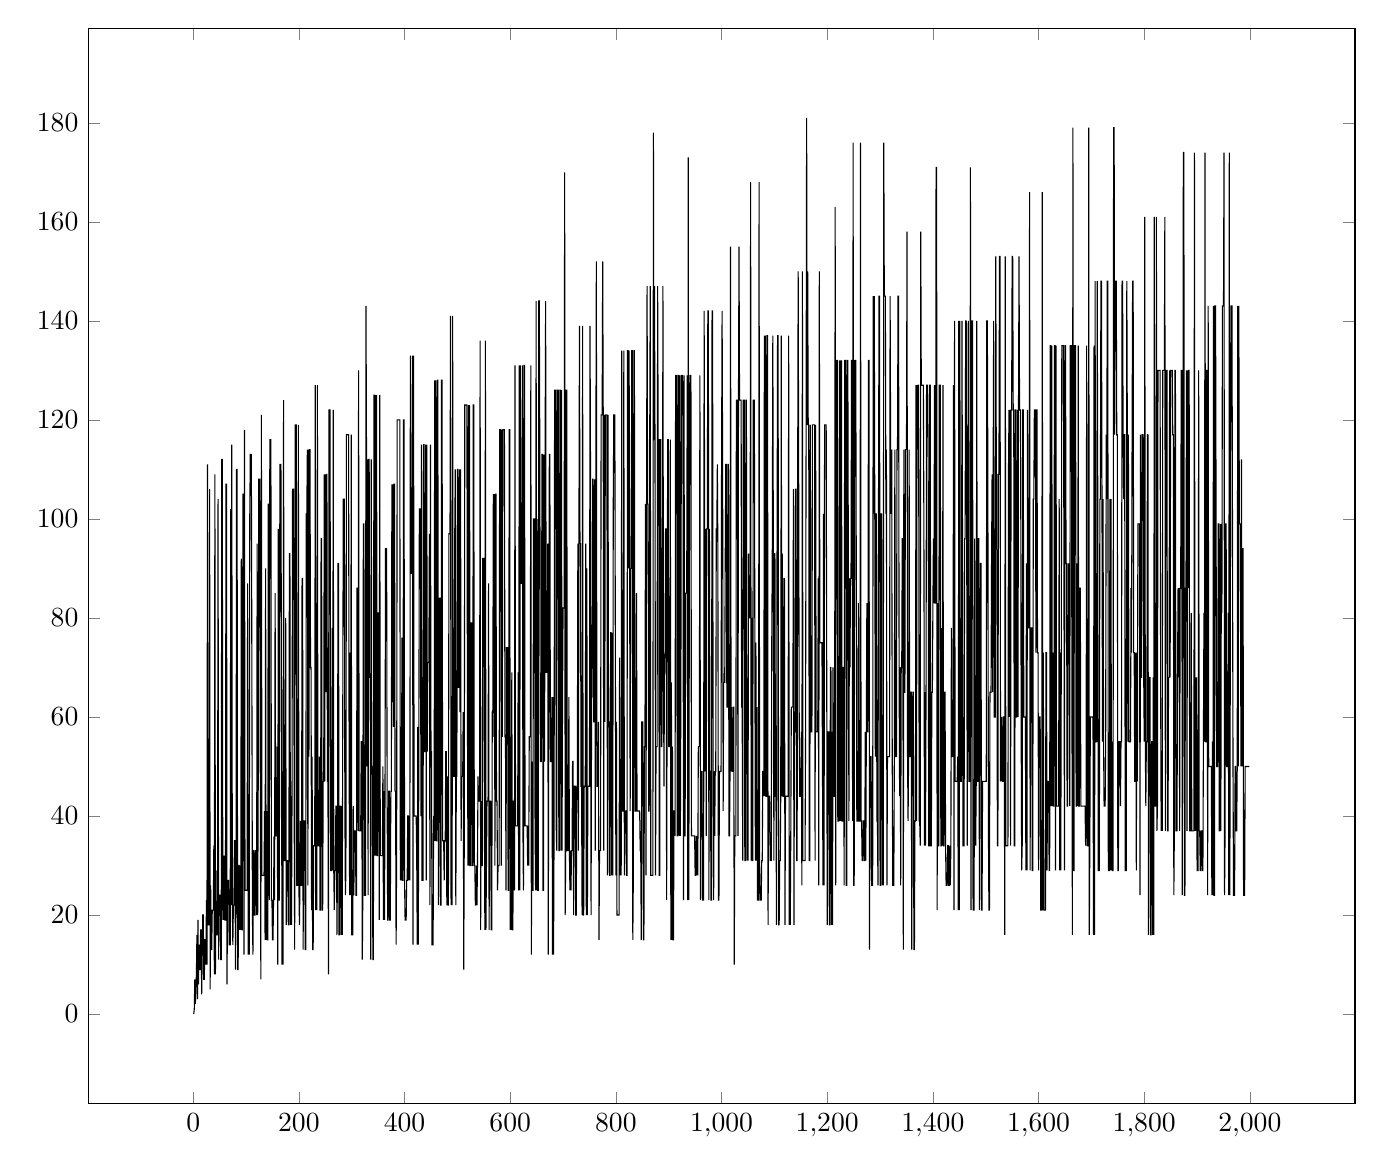
\begin{tikzpicture}
\begin{axis}[height=6in]
\addplot[no markers] coordinates {
(1,0)(2,1)(3,7)(4,2)(5,5)(6,8)(7,16)(8,3)(9,19)(10,6)(11,14)(12,9)(13,9)(14,17)(15,17)(16,4)(17,12)(18,20)(19,20)(20,7)(21,7)(22,15)(23,15)(24,10)(25,23)(26,10)(27,111)(28,18)(29,18)(30,18)(31,106)(32,5)(33,26)(34,13)(35,13)(36,21)(37,21)(38,21)(39,34)(40,8)(41,109)(42,8)(43,29)(44,16)(45,16)(46,16)(47,104)(48,11)(49,24)(50,24)(51,24)(52,11)(53,11)(54,112)(55,112)(56,19)(57,32)(58,19)(59,32)(60,19)(61,19)(62,107)(63,107)(64,6)(65,27)(66,27)(67,27)(68,14)(69,14)(70,14)(71,102)(72,22)(73,115)(74,22)(75,14)(76,22)(77,22)(78,35)(79,35)(80,9)(81,22)(82,110)(83,110)(84,9)(85,9)(86,30)(87,30)(88,17)(89,30)(90,17)(91,92)(92,17)(93,17)(94,105)(95,105)(96,12)(97,118)(98,25)(99,25)(100,25)(101,25)(102,25)(103,87)(104,12)(105,38)(106,12)(107,100)(108,113)(109,113)(110,113)(111,69)(112,20)(113,12)(114,33)(115,33)(116,20)(117,20)(118,33)(119,33)(120,20)(121,95)(122,20)(123,46)(124,108)(125,108)(126,108)(127,46)(128,7)(129,121)(130,28)(131,28)(132,28)(133,28)(134,28)(135,41)(136,15)(137,90)(138,15)(139,41)(140,15)(141,15)(142,103)(143,103)(144,23)(145,116)(146,116)(147,116)(148,23)(149,23)(150,15)(151,15)(152,23)(153,36)(154,23)(155,85)(156,36)(157,36)(158,36)(159,54)(160,10)(161,98)(162,23)(163,23)(164,111)(165,111)(166,111)(167,67)(168,10)(169,49)(170,10)(171,124)(172,31)(173,31)(174,31)(175,80)(176,18)(177,31)(178,31)(179,31)(180,18)(181,18)(182,93)(183,93)(184,18)(185,44)(186,18)(187,44)(188,106)(189,106)(190,106)(191,44)(192,13)(193,119)(194,119)(195,119)(196,26)(197,26)(198,26)(199,119)(200,26)(201,18)(202,26)(203,39)(204,26)(205,26)(206,88)(207,88)(208,13)(209,39)(210,39)(211,39)(212,13)(213,13)(214,101)(215,101)(216,114)(217,26)(218,114)(219,52)(220,114)(221,114)(222,70)(223,70)(224,21)(225,52)(226,13)(227,13)(228,34)(229,34)(230,34)(231,127)(232,21)(233,83)(234,21)(235,127)(236,34)(237,34)(238,34)(239,52)(240,21)(241,21)(242,96)(243,96)(244,21)(245,21)(246,47)(247,47)(248,109)(249,47)(250,109)(251,65)(252,109)(253,109)(254,47)(255,47)(256,8)(257,122)(258,122)(259,122)(260,29)(261,29)(262,29)(263,78)(264,29)(265,122)(266,29)(267,21)(268,29)(269,29)(270,42)(271,42)(272,16)(273,29)(274,91)(275,91)(276,16)(277,16)(278,42)(279,42)(280,16)(281,42)(282,16)(283,60)(284,104)(285,104)(286,104)(287,42)(288,24)(289,29)(290,117)(291,117)(292,117)(293,117)(294,117)(295,55)(296,24)(297,73)(298,24)(299,117)(300,16)(301,16)(302,16)(303,42)(304,24)(305,37)(306,37)(307,37)(308,24)(309,24)(310,86)(311,86)(312,37)(313,130)(314,37)(315,37)(316,37)(317,37)(318,55)(319,55)(320,11)(321,24)(322,99)(323,99)(324,24)(325,24)(326,24)(327,143)(328,112)(329,50)(330,112)(331,24)(332,112)(333,112)(334,68)(335,68)(336,11)(337,112)(338,50)(339,50)(340,11)(341,11)(342,125)(343,125)(344,32)(345,125)(346,32)(347,125)(348,32)(349,32)(350,81)(351,81)(352,19)(353,125)(354,32)(355,32)(356,32)(357,32)(358,32)(359,50)(360,19)(361,45)(362,19)(363,45)(364,94)(365,94)(366,94)(367,45)(368,19)(369,19)(370,45)(371,45)(372,19)(373,19)(374,45)(375,45)(376,107)(377,63)(378,107)(379,58)(380,107)(381,107)(382,45)(383,45)(384,14)(385,32)(386,120)(387,120)(388,120)(389,120)(390,120)(391,120)(392,27)(393,58)(394,27)(395,76)(396,27)(397,27)(398,120)(399,120)(400,27)(401,19)(402,19)(403,19)(404,27)(405,27)(406,40)(407,40)(408,27)(409,40)(410,27)(411,133)(412,89)(413,89)(414,89)(415,133)(416,14)(417,133)(418,40)(419,40)(420,40)(421,40)(422,40)(423,32)(424,14)(425,58)(426,14)(427,53)(428,102)(429,102)(430,102)(431,40)(432,115)(433,27)(434,27)(435,27)(436,115)(437,115)(438,53)(439,53)(440,115)(441,27)(442,115)(443,53)(444,71)(445,71)(446,71)(447,97)(448,22)(449,115)(450,53)(451,53)(452,14)(453,14)(454,14)(455,40)(456,35)(457,128)(458,35)(459,128)(460,35)(461,35)(462,128)(463,128)(464,22)(465,35)(466,84)(467,84)(468,22)(469,22)(470,128)(471,128)(472,35)(473,35)(474,35)(475,27)(476,35)(477,35)(478,53)(479,53)(480,22)(481,48)(482,22)(483,22)(484,97)(485,97)(486,97)(487,141)(488,22)(489,48)(490,22)(491,141)(492,48)(493,48)(494,48)(495,97)(496,110)(497,22)(498,48)(499,48)(500,110)(501,110)(502,66)(503,66)(504,110)(505,61)(506,110)(507,35)(508,48)(509,48)(510,48)(511,61)(512,9)(513,35)(514,123)(515,123)(516,123)(517,123)(518,123)(519,61)(520,30)(521,123)(522,30)(523,123)(524,30)(525,30)(526,79)(527,79)(528,30)(529,30)(530,123)(531,123)(532,30)(533,30)(534,22)(535,22)(536,30)(537,22)(538,30)(539,48)(540,43)(541,43)(542,43)(543,136)(544,17)(545,43)(546,30)(547,30)(548,92)(549,92)(550,92)(551,43)(552,17)(553,136)(554,17)(555,30)(556,43)(557,43)(558,43)(559,87)(560,17)(561,43)(562,43)(563,43)(564,17)(565,17)(566,61)(567,61)(568,105)(569,56)(570,105)(571,30)(572,105)(573,105)(574,43)(575,43)(576,25)(577,30)(578,30)(579,30)(580,118)(581,118)(582,118)(583,30)(584,118)(585,56)(586,118)(587,118)(588,118)(589,118)(590,56)(591,56)(592,25)(593,74)(594,74)(595,74)(596,25)(597,25)(598,118)(599,118)(600,17)(601,56)(602,17)(603,69)(604,17)(605,17)(606,43)(607,43)(608,25)(609,131)(610,38)(611,38)(612,38)(613,38)(614,38)(615,69)(616,25)(617,131)(618,25)(619,131)(620,87)(621,87)(622,87)(623,131)(624,38)(625,25)(626,131)(627,131)(628,38)(629,38)(630,38)(631,38)(632,38)(633,30)(634,38)(635,30)(636,56)(637,56)(638,56)(639,131)(640,12)(641,51)(642,25)(643,25)(644,100)(645,100)(646,100)(647,38)(648,25)(649,144)(650,25)(651,100)(652,25)(653,25)(654,144)(655,144)(656,113)(657,51)(658,51)(659,51)(660,113)(661,113)(662,25)(663,25)(664,113)(665,51)(666,113)(667,144)(668,69)(669,69)(670,69)(671,95)(672,12)(673,64)(674,113)(675,113)(676,51)(677,51)(678,51)(679,64)(680,12)(681,64)(682,12)(683,38)(684,126)(685,126)(686,126)(687,38)(688,33)(689,126)(690,126)(691,126)(692,33)(693,33)(694,126)(695,126)(696,33)(697,126)(698,33)(699,64)(700,82)(701,82)(702,82)(703,170)(704,20)(705,33)(706,126)(707,126)(708,33)(709,33)(710,33)(711,64)(712,33)(713,25)(714,33)(715,25)(716,33)(717,33)(718,51)(719,51)(720,20)(721,46)(722,46)(723,46)(724,20)(725,20)(726,46)(727,46)(728,95)(729,33)(730,95)(731,139)(732,95)(733,95)(734,46)(735,46)(736,20)(737,139)(738,20)(739,20)(740,46)(741,46)(742,46)(743,95)(744,20)(745,90)(746,20)(747,46)(748,46)(749,46)(750,46)(751,139)(752,108)(753,20)(754,64)(755,64)(756,108)(757,108)(758,59)(759,59)(760,108)(761,33)(762,108)(763,152)(764,46)(765,46)(766,46)(767,59)(768,15)(769,33)(770,33)(771,33)(772,121)(773,121)(774,121)(775,152)(776,121)(777,33)(778,121)(779,59)(780,121)(781,121)(782,121)(783,121)(784,28)(785,121)(786,59)(787,59)(788,28)(789,28)(790,77)(791,77)(792,28)(793,77)(794,28)(795,103)(796,121)(797,121)(798,121)(799,72)(800,28)(801,59)(802,20)(803,20)(804,20)(805,20)(806,20)(807,72)(808,28)(809,46)(810,28)(811,134)(812,41)(813,41)(814,41)(815,134)(816,28)(817,41)(818,41)(819,41)(820,28)(821,28)(822,134)(823,134)(824,90)(825,134)(826,90)(827,41)(828,90)(829,90)(830,134)(831,134)(832,15)(833,28)(834,134)(835,134)(836,41)(837,41)(838,41)(839,85)(840,41)(841,41)(842,41)(843,41)(844,41)(845,41)(846,33)(847,33)(848,15)(849,59)(850,59)(851,59)(852,15)(853,15)(854,54)(855,54)(856,103)(857,28)(858,103)(859,147)(860,103)(861,103)(862,41)(863,41)(864,116)(865,147)(866,28)(867,28)(868,28)(869,28)(870,28)(871,178)(872,116)(873,147)(874,116)(875,28)(876,54)(877,54)(878,54)(879,147)(880,116)(881,116)(882,28)(883,28)(884,116)(885,116)(886,54)(887,54)(888,72)(889,147)(890,72)(891,46)(892,72)(893,72)(894,98)(895,98)(896,23)(897,67)(898,116)(899,116)(900,54)(901,54)(902,54)(903,116)(904,15)(905,67)(906,15)(907,54)(908,15)(909,15)(910,41)(911,41)(912,36)(913,129)(914,129)(915,129)(916,36)(917,36)(918,129)(919,129)(920,36)(921,129)(922,36)(923,67)(924,129)(925,129)(926,129)(927,116)(928,23)(929,129)(930,36)(931,36)(932,85)(933,85)(934,85)(935,129)(936,23)(937,173)(938,23)(939,85)(940,129)(941,129)(942,129)(943,36)(944,36)(945,36)(946,36)(947,36)(948,36)(949,36)(950,28)(951,28)(952,36)(953,28)(954,36)(955,28)(956,54)(957,54)(958,54)(959,129)(960,23)(961,49)(962,49)(963,49)(964,23)(965,23)(966,23)(967,142)(968,98)(969,49)(970,98)(971,36)(972,98)(973,98)(974,142)(975,142)(976,23)(977,98)(978,49)(979,49)(980,23)(981,23)(982,142)(983,142)(984,49)(985,23)(986,49)(987,36)(988,49)(989,49)(990,98)(991,98)(992,111)(993,93)(994,23)(995,23)(996,49)(997,49)(998,49)(999,49)(1000,111)(1001,142)(1002,111)(1003,41)(1004,67)(1005,67)(1006,67)(1007,93)(1008,111)(1009,111)(1010,62)(1011,62)(1012,111)(1013,111)(1014,36)(1015,36)(1016,49)(1017,155)(1018,49)(1019,62)(1020,49)(1021,49)(1022,62)(1023,62)(1024,10)(1025,36)(1026,36)(1027,36)(1028,124)(1029,124)(1030,124)(1031,36)(1032,124)(1033,155)(1034,124)(1035,124)(1036,124)(1037,124)(1038,62)(1039,62)(1040,31)(1041,124)(1042,124)(1043,124)(1044,31)(1045,31)(1046,124)(1047,124)(1048,31)(1049,62)(1050,31)(1051,93)(1052,80)(1053,80)(1054,80)(1055,168)(1056,31)(1057,80)(1058,31)(1059,31)(1060,124)(1061,124)(1062,124)(1063,75)(1064,31)(1065,75)(1066,31)(1067,62)(1068,23)(1069,23)(1070,23)(1071,168)(1072,31)(1073,23)(1074,23)(1075,23)(1076,31)(1077,31)(1078,49)(1079,49)(1080,44)(1081,137)(1082,44)(1083,137)(1084,44)(1085,44)(1086,137)(1087,137)(1088,18)(1089,44)(1090,44)(1091,44)(1092,31)(1093,31)(1094,31)(1095,75)(1096,93)(1097,137)(1098,93)(1099,31)(1100,93)(1101,93)(1102,44)(1103,44)(1104,18)(1105,93)(1106,137)(1107,137)(1108,18)(1109,18)(1110,31)(1111,31)(1112,44)(1113,137)(1114,44)(1115,93)(1116,44)(1117,44)(1118,88)(1119,88)(1120,18)(1121,44)(1122,44)(1123,44)(1124,44)(1125,44)(1126,44)(1127,137)(1128,18)(1129,36)(1130,18)(1131,36)(1132,62)(1133,62)(1134,62)(1135,62)(1136,106)(1137,18)(1138,57)(1139,57)(1140,106)(1141,106)(1142,31)(1143,31)(1144,106)(1145,150)(1146,106)(1147,57)(1148,44)(1149,44)(1150,44)(1151,57)(1152,26)(1153,150)(1154,31)(1155,31)(1156,31)(1157,31)(1158,31)(1159,57)(1160,119)(1161,181)(1162,119)(1163,150)(1164,119)(1165,119)(1166,31)(1167,31)(1168,119)(1169,57)(1170,57)(1171,57)(1172,119)(1173,119)(1174,119)(1175,119)(1176,119)(1177,31)(1178,119)(1179,57)(1180,57)(1181,57)(1182,57)(1183,88)(1184,26)(1185,150)(1186,75)(1187,75)(1188,75)(1189,75)(1190,75)(1191,49)(1192,26)(1193,101)(1194,26)(1195,119)(1196,119)(1197,119)(1198,119)(1199,70)(1200,18)(1201,57)(1202,57)(1203,57)(1204,18)(1205,18)(1206,70)(1207,70)(1208,18)(1209,57)(1210,18)(1211,70)(1212,44)(1213,44)(1214,44)(1215,163)(1216,26)(1217,132)(1218,132)(1219,132)(1220,39)(1221,39)(1222,39)(1223,132)(1224,39)(1225,132)(1226,39)(1227,132)(1228,39)(1229,39)(1230,70)(1231,70)(1232,26)(1233,132)(1234,132)(1235,132)(1236,26)(1237,26)(1238,132)(1239,132)(1240,88)(1241,39)(1242,88)(1243,70)(1244,88)(1245,88)(1246,132)(1247,132)(1248,39)(1249,176)(1250,26)(1251,26)(1252,132)(1253,132)(1254,132)(1255,88)(1256,39)(1257,39)(1258,39)(1259,83)(1260,39)(1261,39)(1262,39)(1263,176)(1264,39)(1265,39)(1266,31)(1267,31)(1268,39)(1269,39)(1270,31)(1271,31)(1272,57)(1273,31)(1274,57)(1275,83)(1276,57)(1277,57)(1278,132)(1279,132)(1280,13)(1281,52)(1282,52)(1283,52)(1284,26)(1285,26)(1286,26)(1287,145)(1288,101)(1289,145)(1290,101)(1291,52)(1292,101)(1293,101)(1294,39)(1295,39)(1296,26)(1297,101)(1298,145)(1299,145)(1300,26)(1301,26)(1302,101)(1303,101)(1304,26)(1305,52)(1306,26)(1307,176)(1308,145)(1309,145)(1310,145)(1311,101)(1312,114)(1313,26)(1314,52)(1315,52)(1316,52)(1317,52)(1318,52)(1319,145)(1320,114)(1321,101)(1322,114)(1323,52)(1324,26)(1325,26)(1326,26)(1327,52)(1328,114)(1329,52)(1330,52)(1331,52)(1332,114)(1333,114)(1334,145)(1335,145)(1336,70)(1337,44)(1338,70)(1339,26)(1340,70)(1341,70)(1342,96)(1343,96)(1344,13)(1345,114)(1346,65)(1347,65)(1348,114)(1349,114)(1350,114)(1351,158)(1352,52)(1353,39)(1354,52)(1355,114)(1356,52)(1357,52)(1358,65)(1359,65)(1360,13)(1361,52)(1362,65)(1363,65)(1364,13)(1365,13)(1366,39)(1367,39)(1368,127)(1369,39)(1370,127)(1371,114)(1372,127)(1373,127)(1374,39)(1375,39)(1376,34)(1377,158)(1378,127)(1379,127)(1380,127)(1381,127)(1382,127)(1383,96)(1384,34)(1385,65)(1386,34)(1387,65)(1388,127)(1389,127)(1390,127)(1391,114)(1392,34)(1393,34)(1394,127)(1395,127)(1396,34)(1397,34)(1398,65)(1399,65)(1400,83)(1401,96)(1402,83)(1403,127)(1404,83)(1405,83)(1406,171)(1407,171)(1408,21)(1409,83)(1410,34)(1411,34)(1412,127)(1413,127)(1414,127)(1415,34)(1416,34)(1417,78)(1418,34)(1419,127)(1420,34)(1421,34)(1422,65)(1423,65)(1424,34)(1425,26)(1426,26)(1427,26)(1428,34)(1429,34)(1430,26)(1431,26)(1432,34)(1433,26)(1434,34)(1435,78)(1436,52)(1437,52)(1438,52)(1439,127)(1440,21)(1441,140)(1442,47)(1443,47)(1444,47)(1445,47)(1446,47)(1447,52)(1448,21)(1449,140)(1450,21)(1451,140)(1452,47)(1453,47)(1454,47)(1455,140)(1456,96)(1457,34)(1458,34)(1459,34)(1460,96)(1461,96)(1462,140)(1463,140)(1464,96)(1465,34)(1466,96)(1467,140)(1468,47)(1469,47)(1470,47)(1471,171)(1472,21)(1473,96)(1474,140)(1475,140)(1476,21)(1477,21)(1478,21)(1479,96)(1480,47)(1481,34)(1482,47)(1483,140)(1484,47)(1485,47)(1486,96)(1487,96)(1488,21)(1489,47)(1490,91)(1491,91)(1492,21)(1493,21)(1494,47)(1495,47)(1496,47)(1497,47)(1498,47)(1499,47)(1500,47)(1501,47)(1502,140)(1503,140)(1504,109)(1505,39)(1506,21)(1507,21)(1508,65)(1509,65)(1510,65)(1511,91)(1512,109)(1513,65)(1514,109)(1515,140)(1516,60)(1517,60)(1518,60)(1519,153)(1520,109)(1521,109)(1522,34)(1523,34)(1524,109)(1525,109)(1526,153)(1527,153)(1528,47)(1529,60)(1530,47)(1531,60)(1532,47)(1533,47)(1534,60)(1535,60)(1536,16)(1537,153)(1538,34)(1539,34)(1540,34)(1541,34)(1542,34)(1543,109)(1544,122)(1545,60)(1546,122)(1547,34)(1548,122)(1549,122)(1550,153)(1551,153)(1552,122)(1553,122)(1554,34)(1555,34)(1556,122)(1557,122)(1558,60)(1559,60)(1560,122)(1561,60)(1562,122)(1563,153)(1564,122)(1565,122)(1566,122)(1567,60)(1568,29)(1569,34)(1570,122)(1571,122)(1572,60)(1573,60)(1574,60)(1575,60)(1576,29)(1577,91)(1578,29)(1579,122)(1580,78)(1581,78)(1582,78)(1583,166)(1584,29)(1585,78)(1586,78)(1587,78)(1588,29)(1589,29)(1590,104)(1591,104)(1592,122)(1593,122)(1594,122)(1595,73)(1596,122)(1597,122)(1598,73)(1599,73)(1600,29)(1601,60)(1602,60)(1603,60)(1604,21)(1605,21)(1606,21)(1607,166)(1608,21)(1609,73)(1610,21)(1611,21)(1612,21)(1613,21)(1614,73)(1615,73)(1616,29)(1617,47)(1618,47)(1619,47)(1620,29)(1621,29)(1622,135)(1623,135)(1624,42)(1625,135)(1626,42)(1627,73)(1628,42)(1629,42)(1630,135)(1631,135)(1632,29)(1633,135)(1634,42)(1635,42)(1636,42)(1637,42)(1638,42)(1639,104)(1640,29)(1641,73)(1642,29)(1643,73)(1644,135)(1645,135)(1646,135)(1647,135)(1648,91)(1649,29)(1650,135)(1651,135)(1652,91)(1653,91)(1654,42)(1655,42)(1656,91)(1657,73)(1658,91)(1659,42)(1660,135)(1661,135)(1662,135)(1663,73)(1664,16)(1665,179)(1666,29)(1667,29)(1668,135)(1669,135)(1670,135)(1671,42)(1672,42)(1673,91)(1674,42)(1675,135)(1676,42)(1677,42)(1678,86)(1679,86)(1680,42)(1681,42)(1682,42)(1683,42)(1684,42)(1685,42)(1686,42)(1687,42)(1688,42)(1689,34)(1690,42)(1691,135)(1692,34)(1693,34)(1694,34)(1695,179)(1696,16)(1697,34)(1698,60)(1699,60)(1700,60)(1701,60)(1702,60)(1703,60)(1704,16)(1705,135)(1706,16)(1707,148)(1708,55)(1709,55)(1710,55)(1711,148)(1712,104)(1713,29)(1714,29)(1715,29)(1716,104)(1717,104)(1718,148)(1719,148)(1720,104)(1721,55)(1722,104)(1723,55)(1724,42)(1725,42)(1726,42)(1727,55)(1728,117)(1729,104)(1730,148)(1731,148)(1732,29)(1733,29)(1734,29)(1735,104)(1736,29)(1737,104)(1738,29)(1739,55)(1740,29)(1741,29)(1742,179)(1743,179)(1744,117)(1745,148)(1746,148)(1747,148)(1748,117)(1749,117)(1750,29)(1751,29)(1752,55)(1753,55)(1754,55)(1755,42)(1756,55)(1757,55)(1758,148)(1759,148)(1760,117)(1761,104)(1762,117)(1763,117)(1764,29)(1765,29)(1766,29)(1767,148)(1768,117)(1769,55)(1770,117)(1771,55)(1772,55)(1773,55)(1774,55)(1775,86)(1776,73)(1777,117)(1778,148)(1779,148)(1780,73)(1781,73)(1782,47)(1783,47)(1784,73)(1785,29)(1786,73)(1787,47)(1788,99)(1789,99)(1790,99)(1791,99)(1792,24)(1793,117)(1794,68)(1795,68)(1796,117)(1797,117)(1798,117)(1799,68)(1800,55)(1801,161)(1802,55)(1803,42)(1804,55)(1805,55)(1806,117)(1807,117)(1808,16)(1809,55)(1810,68)(1811,68)(1812,16)(1813,16)(1814,55)(1815,55)(1816,16)(1817,68)(1818,16)(1819,161)(1820,42)(1821,42)(1822,42)(1823,161)(1824,37)(1825,42)(1826,130)(1827,130)(1828,130)(1829,130)(1830,130)(1831,68)(1832,37)(1833,42)(1834,37)(1835,130)(1836,130)(1837,130)(1838,130)(1839,161)(1840,37)(1841,130)(1842,130)(1843,130)(1844,37)(1845,37)(1846,68)(1847,68)(1848,130)(1849,68)(1850,130)(1851,130)(1852,130)(1853,130)(1854,117)(1855,117)(1856,24)(1857,37)(1858,130)(1859,130)(1860,37)(1861,37)(1862,37)(1863,68)(1864,86)(1865,68)(1866,86)(1867,37)(1868,86)(1869,86)(1870,130)(1871,130)(1872,24)(1873,86)(1874,174)(1875,174)(1876,24)(1877,24)(1878,86)(1879,86)(1880,130)(1881,37)(1882,130)(1883,86)(1884,130)(1885,130)(1886,37)(1887,37)(1888,37)(1889,81)(1890,37)(1891,37)(1892,37)(1893,37)(1894,37)(1895,174)(1896,37)(1897,68)(1898,37)(1899,68)(1900,29)(1901,29)(1902,29)(1903,130)(1904,37)(1905,37)(1906,29)(1907,29)(1908,37)(1909,37)(1910,29)(1911,29)(1912,55)(1913,81)(1914,55)(1915,174)(1916,55)(1917,55)(1918,130)(1919,130)(1920,24)(1921,143)(1922,50)(1923,50)(1924,50)(1925,50)(1926,50)(1927,50)(1928,24)(1929,55)(1930,24)(1931,143)(1932,24)(1933,24)(1934,143)(1935,143)(1936,99)(1937,50)(1938,50)(1939,50)(1940,99)(1941,99)(1942,37)(1943,37)(1944,99)(1945,37)(1946,99)(1947,81)(1948,143)(1949,143)(1950,143)(1951,174)(1952,24)(1953,37)(1954,99)(1955,99)(1956,50)(1957,50)(1958,50)(1959,81)(1960,24)(1961,174)(1962,24)(1963,81)(1964,143)(1965,143)(1966,143)(1967,99)(1968,50)(1969,24)(1970,24)(1971,24)(1972,50)(1973,50)(1974,37)(1975,37)(1976,50)(1977,143)(1978,50)(1979,143)(1980,99)(1981,99)(1982,99)(1983,50)(1984,112)(1985,50)(1986,94)(1987,94)(1988,24)(1989,24)(1990,24)(1991,50)(1992,50)(1993,50)(1994,50)(1995,50)(1996,50)(1997,50)(1998,50)(1999,50)
};
\end{axis}
\end{tikzpicture}
\end{center}

I hope that it's clear at least that
the number of iterations for $n = 2^k$
is $k$.
These are the optimistic cases.
Do you see why?

I'll leave it to you to play around with the above while-loop.

